\documentclass[11pt, oneside]{article}   	% use "amsart" instead of "article" for AMSLaTeX format
\usepackage{geometry}                		% See geometry.pdf to learn the layout options. There are lots.
\geometry{letterpaper}                   		% ... or a4paper or a5paper or ... 
%\geometry{landscape}                		% Activate for for rotated page geometry
%\usepackage[parfill]{parskip}    		% Activate to begin paragraphs with an empty line rather than an indent
\usepackage{graphicx}				% Use pdf, png, jpg, or eps� with pdflatex; use eps in DVI mode
								% TeX will automatically convert eps --> pdf in pdflatex		
\usepackage{amssymb}
\usepackage{amsmath}
\usepackage{parskip}
\usepackage{color}

\title{Divergence}
%\author{The Author}
%\section{}
% \subsection*{R code}
\date{}							% Activate to display a given date or no date

\graphicspath{{/Users/telliott_admin/Dropbox/Tex/png/}}

% \begin{center} 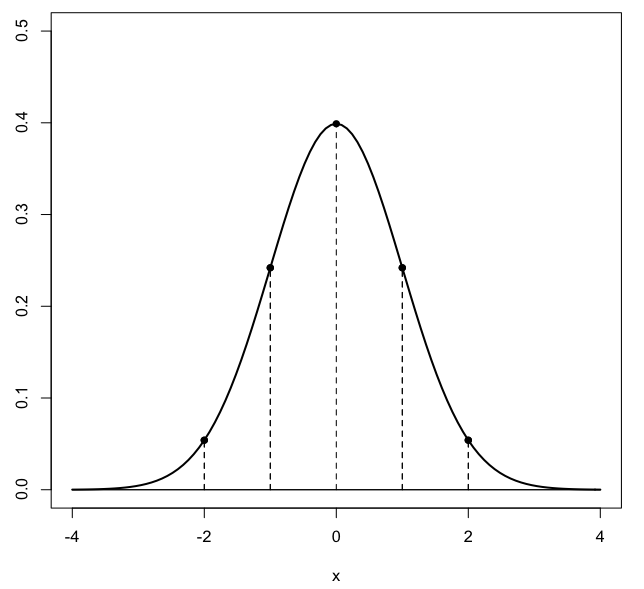
\includegraphics [scale=0.4] {gauss3.png} \end{center}
% \begin{bmatrix} a  &  b \\ c  &  d \end{bmatrix}
% \bigg |_

\begin{document}
\maketitle
\large
%\noindent
\subsection*{Divergence and curl}
The "del" operator
\[ \nabla = \ < \frac{\partial}{\partial x},\frac{\partial}{\partial y},\frac{\partial}{\partial z} > \]
The divergence of $\mathbf{F}$ is
\[ \nabla \cdot \mathbf{F} \]
if $\mathbf{F} = \ <P,Q,R>$
\[ \nabla \cdot \mathbf{F} = P_x + Q_y + R_z \]
The divergence of a vector field is a scalar quantity.

The curl of $\mathbf{F}$ is
\[ \nabla \times \mathbf{F} \]
if $\mathbf{F} = \ <P,Q,R>$
\[ \nabla \times \mathbf{F} =  \ <R_y-Q_z,P_z-R_x,Q_x-P_y> \]
which is basically impossible to remember, but using this convenient device
\[
\begin{vmatrix} 
  \hat{i}  &  \hat{j} & \hat{k} \\ 
  \frac{\partial}{\partial x}  &  \frac{\partial}{\partial y} & \frac{\partial}{\partial z} \\ 
  P  &  Q & R \\ 
\end{vmatrix} \ \ 
\]
it's a lot easier.
\subsection*{Green's Theorem}
The work done moving along a curve is
\[ W = \int_C \mathbf{F} \cdot d\mathbf{r}  = \int_C \mathbf{F} \cdot \hat{\mathbf{T}} \ ds \]
In the plane, the theorem states that for a closed path
\[ \oint \mathbf{F} \cdot d\mathbf{r}  = \iint_R \ \nabla \times \mathbf{F} \]
The work done along a closed path around $R$ is equal to the integral over $R$ of the curl of $\mathbf{F}$.

Restated
\[ \int_C M \ dx + N \ dy = \iint_R \ (N_x - M_y) \ dA \]
One sticky point I had here is that the curl produces a vector, yet the formula is usually given as above.  That's because this is a special case of Stokes theorem where the term on the right is really 
\[ (\nabla \times \mathbf{F}) \cdot \hat{\mathbf{k}} \ dA \]
which (since $\nabla \times \mathbf{F} $ is parallel to $\hat{\mathbf{k}}$) gives what we have above.

The other form of Green is for the flux
\[ \oint \mathbf{F} \cdot \hat{\mathbf{n}} \ ds  = \iint_R \ \nabla \cdot \mathbf{F} \]
The flux across a closed path around $R$ is equal to the integral over $R$ of the divergence of $\mathbf{F}$.

Restated
\[ \int_C -N \ dx + M \ dy = \iint_R \ (M_x + N_y) \ dA \]

There is another theorem called the divergence theorem which is also called Gauss's Theorem (and some other people's names too), that is basically the 3D version of the flux form of Green's Theorem.  Auroux calls it "Green's Theorem in Space."  The flux across a closed surface in space

\[ \iint_S \mathbf{F} \cdot \hat{\mathbf{n}} \ dS  = \iiint_R \ \nabla \cdot \mathbf{F} \]

\subsection*{Divergence in other coordinate systems}
The "del" operator is
\[ \nabla = \ < \frac{\partial}{\partial x},\frac{\partial}{\partial y},\frac{\partial}{\partial z} > \]
The divergence of $\mathbf{F}$ is
\[ \nabla \cdot \mathbf{F} \]
if $\mathbf{F} = \ <P,Q,R>$
\[ \nabla \cdot \mathbf{F} = P_x + Q_y + R_z \]
The divergence of a vector field is a scalar quantity.

In cylindrical and spherical coordinates, the divergence is more complicated.  Although the expression above is often given as the \emph{definition} of divergence, Schey makes a big deal out of saying that he prefers this definition

\[ div \mathbf{F} = \lim_{\Delta V \rightarrow 0} \frac{1}{\Delta V} \iint_S \ \mathbf{F} \cdot \hat{\mathbf{n}} \ dS \]

As further illustration, the divergence has a more complicated form in cylindrical and spherical coordinates.  In the former it is 

\[ div \mathbf{\mathbf{F}} = \frac{1}{r} \frac{\partial}{\partial r} (rF_r) +  \frac{1}{r} \frac{\partial}{\partial \theta} (F_{\theta}) + \frac{\partial}{\partial z} (F_z) \]

where $F_{z}$ is not a partial derivative but just the component of $\mathbf{F}$ in the z-direction, and so on.

Similarly, in spherical coordinates the divergence is

\[ div \mathbf{\mathbf{F}} = \frac{1}{r^2} \frac{\partial}{\partial r} (r^2F_r) +  \frac{1}{r \ \sin \phi} \frac{\partial}{\partial \phi} (\sin \phi F_{\phi}) + \frac{1}{r \ \sin \phi} \frac{\partial}{\partial \theta} (F_{\theta}) \]

\subsection*{Stokes}

\[ \oint_C \mathbf{F} \cdot d \mathbf{r} = \iint_S ( \nabla \times \mathbf{F}) \cdot \mathbf{n} \ dS \]
Stokes theorem applies to a curve in space (I'm not sure at the moment whether it has to lie in a plane or not).  It says that the work going around the curve is equal to the integral over \emph{any surface} with that curve as its boundary of the flux of the curl of $\mathbf{F}$. 

\end{document}  